
%==============%
\section{非言語大学}
%=============%
非言語大学(Higengo University、以下 HU)は、国際的な非言語研究機関であり、全世界人口のうち約50億人が入学希望を出している(入学希望は0.000001パーセントの確率で受理される)。
HUの研究員は非言語研究を通じ、全世界から戦争を無くし平和な世の中になればいいなと思っているが、予算の都合上行動に起こせていない。税金を投入すべきである。
非言語大学は、非言語大学相当研究室まがいのプレハブ小屋として全世界に拠点を置いているが、特にアバリカ合衆国ニューイヨォクに拠点を置く「意味のNASA」は、宇宙開発計画および宇宙開発産業、航空研究などの中心機関として活躍しているNASAに劣っており、意味がない。
以上の様に、非言語大学は予算の都合上一切役割を果たせていない研究室をおよそ100000個抱えており、全世界からの寄付を求めている。
\par
この様に経営に難を抱えている状況を打破するために非言語大学本部は、国際高等研究所アバラ連携宇宙研究機構 (Abara Univ.) で2007年10月1日から11年14日間にわたり機構長を務めてきた武田初代機構長を本部へ移動させることにした。
これに伴い、アバラ連携宇宙研究機構は消滅した。
移動に伴いアバラ宇宙研究機構を潰した責務により武田機構長は非言語大学事務方により起訴され、懲役100万光年の系に処している。
そこで、非言語大学新機構長としてカリフォルニア工科大学教授を兼任していたギャラクシー・アバラボネを抜擢することにした。
本章では入学要項を読み解くことで、非言語大学の機構長に誰を選抜すべきか、どのような条件を用いれば非言語大学の経営が上向くかを研究した。

%~~~~~~~~~~~~~~~~~~~~~~~~~%
\subsection{非言語大学の歴史}
%~~~~~~~~~~~~~~~~~~~~~~~~~%
非言語大学が発足するとなったきっかけは、初代非言語大学機構長である竹田総理、初代総務大臣小川の出会いである。
2012年イノシシ大学に入城したお二方は、4月の段階では実はまだ出会ってないに等しかったのである。
初代機構長は様々な新歓を渡り歩き、初代総務大臣はCSC(?)を渡り歩いていた。
そのようにあまり混じり合わなかった二人をひきつけたのはかの有名な「出会いのインターフェース」ことファンファン亭ヨネスケ大師匠である。

%========================%
\subsubsection{初代機構長的観点}
%========================%
竹田機構長は2012年の4月に物理学部として図●●の集合写真を撮った。
% ----- 集合写真が欲しい。
この時にはカメラマンの方から「XX君はここに並んで、△△君はここに並んで、・・・」と指示が飛んでいた。
その中で機構長の耳にふと「ファン君は〜」と飛び込んできたのである。
ここで機構長がインターフェースを取得した瞬間である。
つまり他の学生の名前は覚えれなかったが、ファンファン亭ヨネスケの名前は特別すぎて覚えることに成功したのである。
この集合写真のあと、何らかのガイダンスがあり、色々と話しを聞いた。思い出すと、機構長がガッツリ最初に話しかけたのは横にいたウエーバー君であった。(ポ)「高校まで何してたん?」(Wb)「バスケ...。」この後、6年間、コレ以上の会話をしていない。
そしてガイダンス後、特に友人のできなかった機構長は帰ろうとして、LANS生協の横を通り帰ろうとした瞬間、ヨネスケ師匠が通ったのである。
ここで機構長の友人作成スイッチが入りヨネスケ師匠に話しかけた。
今でも鮮明に覚えているが、「通学証明書発行機ってどこ?」と話しかけた。
これがインターフェース獲得の瞬間である。
今後このインターフェースを通じ、自宅で鍋をし、永遠とティッシュで野球をした。このときに、初代総務大臣は盛大にパーティーピーポーとなった。
\par
記憶の最初は、ヨネヨネCLUB創設である。
阪急電車十三駅で特急に乗り換えているときに「Wikipediaでリンクを辿っていけば絶対に自分の行きたいページにいける」というネタをひっさげてお互い喋っていた。
そのときに初代機構長が「こういうネタあるよ、小川くんの好きなものはなに?」という答えに対し「EXILE」であると答えたことが未だに記憶に残っている。
案の定、任意のページからEXILEに辿り着き、まぁまぁ初対面ながら間がもったのは覚えている。

%========================%
\subsubsection{LIFE的観点}
%========================%
学部生3回生の頃の初代機構長はバイト先に困っていた。
そのところに、小川総務大臣の助言によりライフで働くことになった。なんとなくレジに興味あると言って、なんとなくレジ部門になった。半額ボタンを押して色々買ったり、買い物に来た宮崎大輔のコメを半額にしてやった。ある程度してやめた。
ここから俗に言うデブ活が更に加速していったのである。
%\begin{figure}
%\centering
%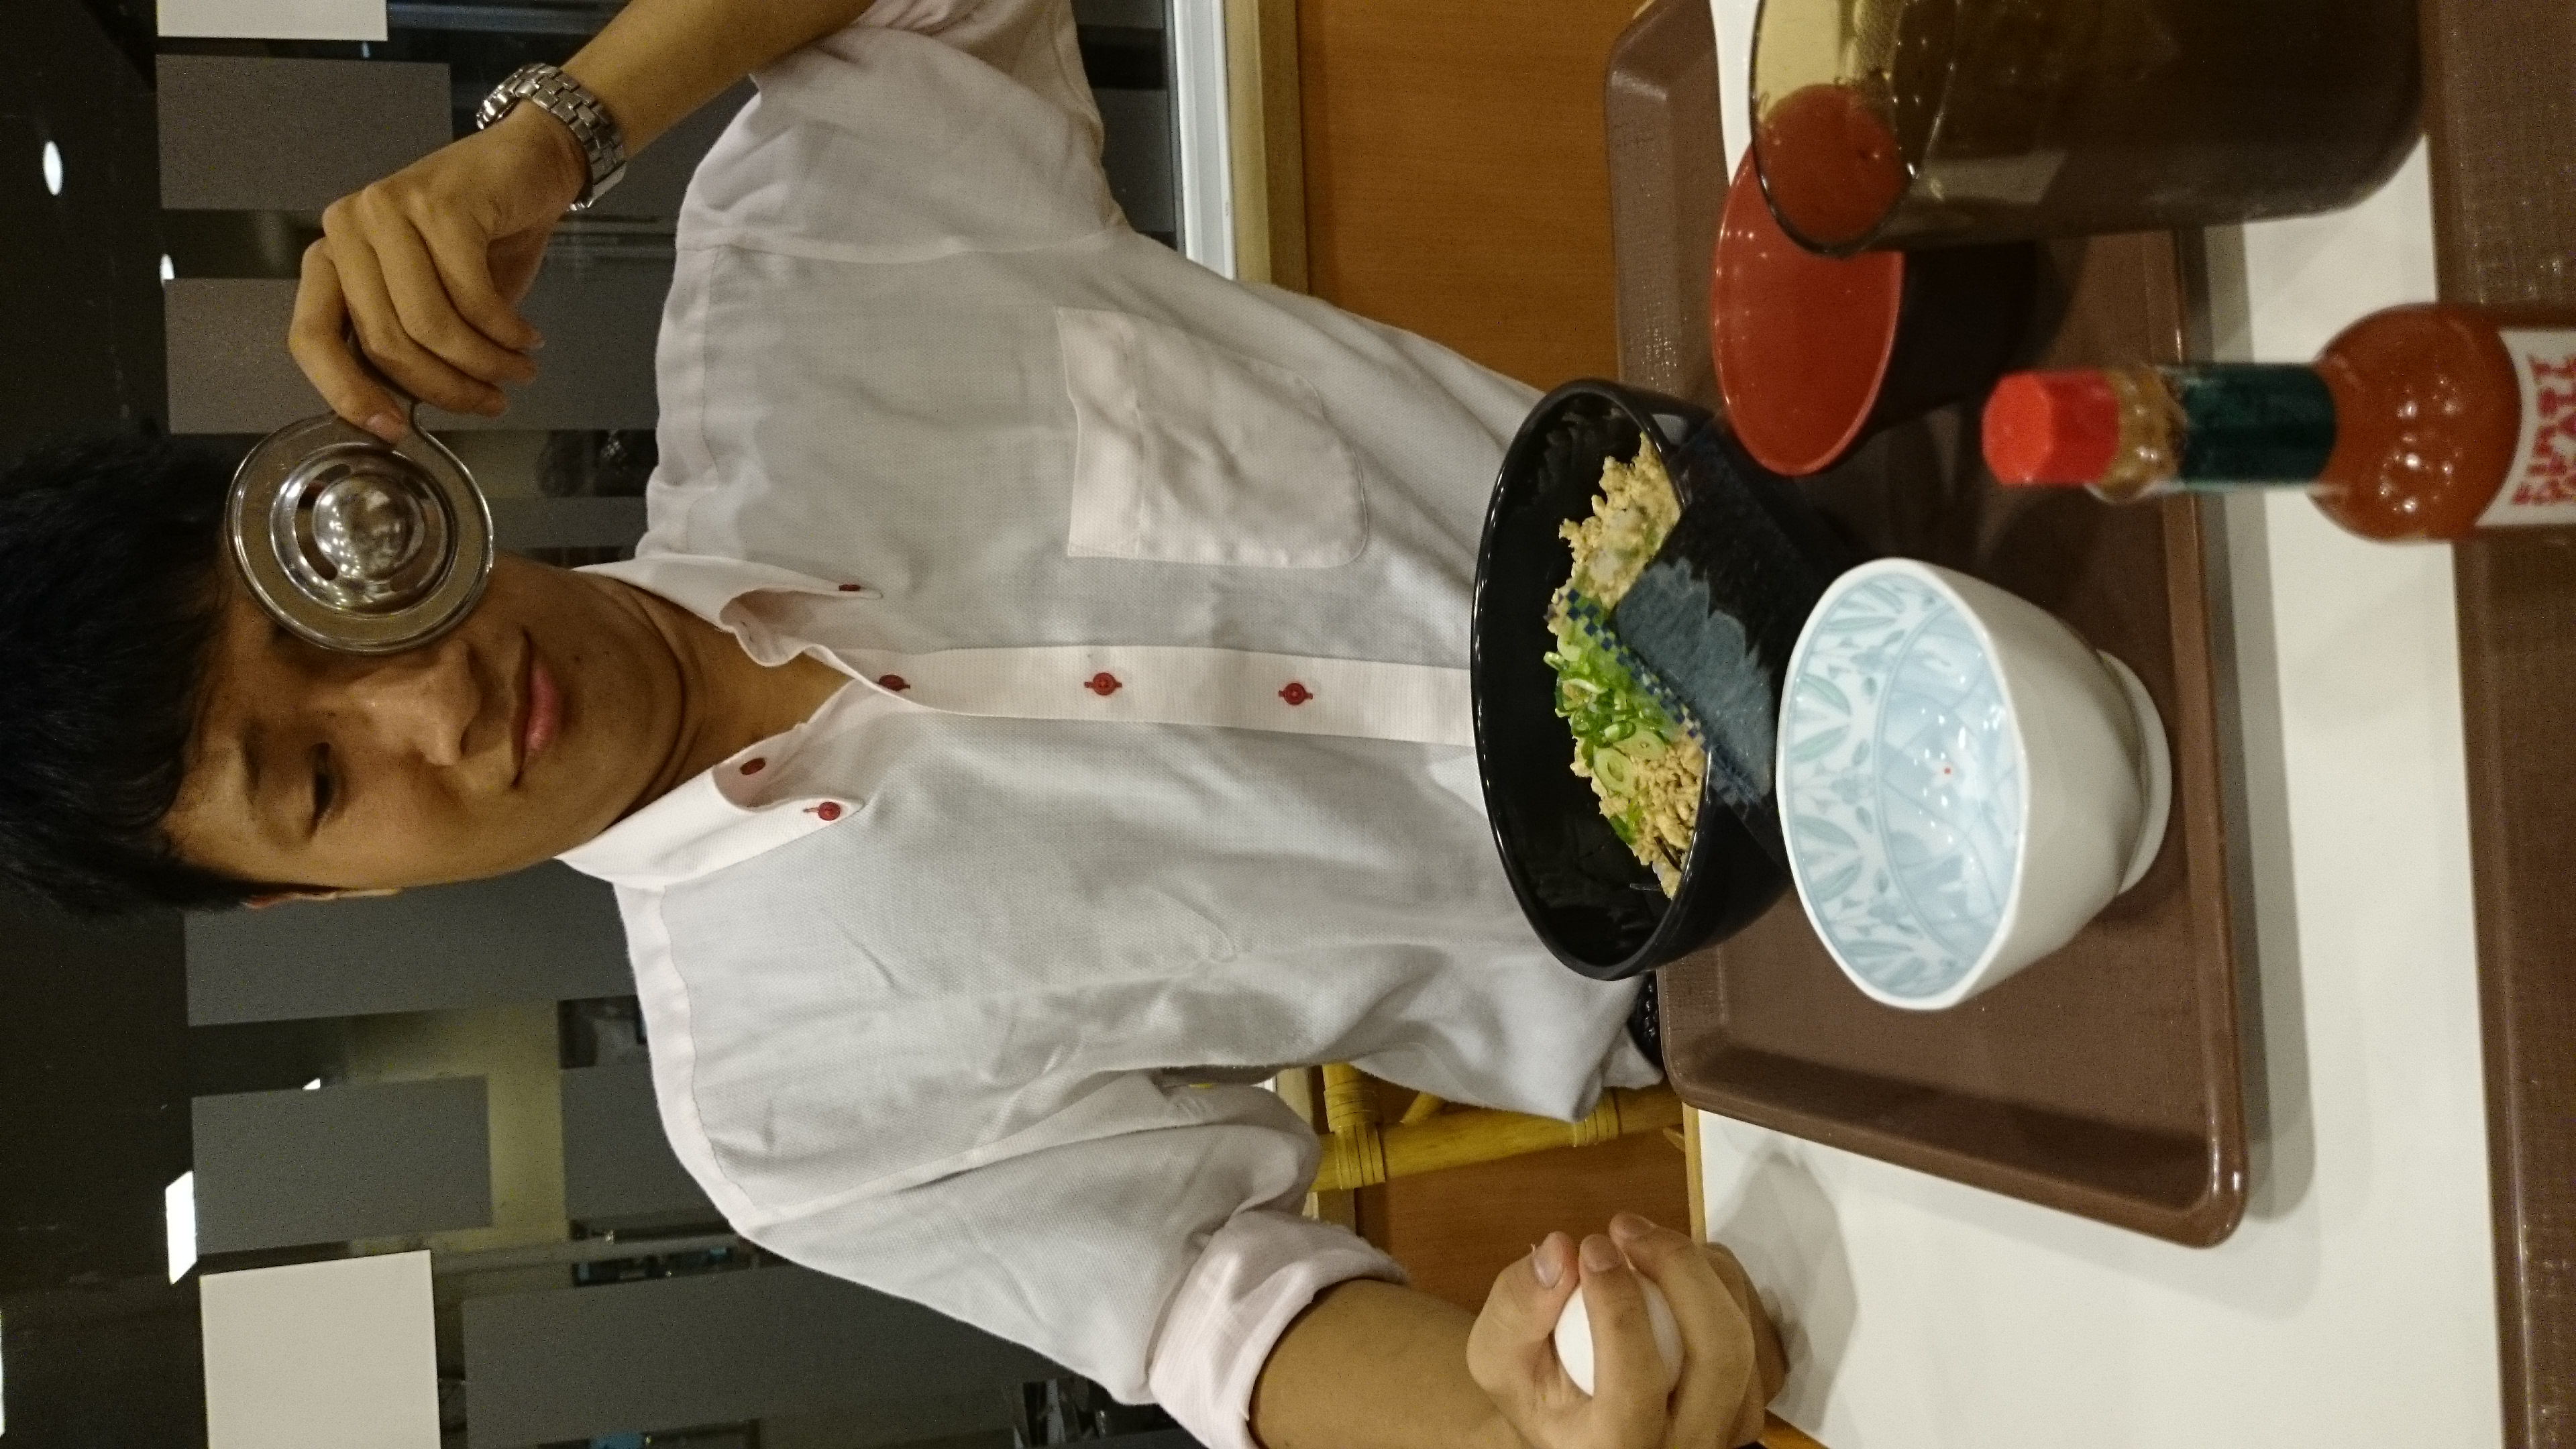
\includegraphics[scale=0.3]{figures/DebuKatsu}
%\caption{ライフ近くの晩ごはん屋さん。}
%\label{mimi}
%\end{figure}


%~~~~~~~~~~~~~~~~~~~~~~~~~~~~~~~~~~~~~~~~~~~~~~~%
\subsection{非言語大学相当研究室のようなプレハブ小屋について}
%~~~~~~~~~~~~~~~~~~~~~~~~~~~~~~~~~~~~~~~~~~~~%
非言語大学相当の研究室約1000000研究室は文部科学省の世界トップレベル国際研究拠点形成促進プログラムに採択され、数学、物理、天文学の3分野の連携による融合研究を行いながら、国内外の研究者や一般の方へも認知される国際的な研究所として成長してきた。
2012年4月にはニュウイヨォク米国財団の寄附を受け、非言語大学国際高等研究所アブラ数物連携宇宙研究機構へと改称された後、約999999研究室が廃部・統合、一つのアブラ研究所となった。
非言語大学国際高等研究所アブラ研究機構は、文部科学省の世界トップレベル国際研究拠点形成促進プログラムに採択され、2007年10月1日に非言語大学数物連携宇宙研究機構として9年半の時限付き研究所として発足した。
「非言語はどうやって始まったのか、その運命は何か、何で出来ているのか、どういう法則に支配されていて、なぜ我々は存在するのか」と言った小川・竹田が入学以来問い続けてきた宇宙の最も根本的な謎を解明するため、数学、物理、天文学の3分野が分野の枠を超えて研究を行ってきた。
毎日平日15時に開催される研究者の集う温泉入浴時間、数多くの国際会議の開催等、融合研究を促進する環境が契機となり世界に認められる研究成果を数多く生み出して来た。
それが優秀な人材が世界中から更に集まる好循環となり、人も建物もゼロから始まった弊機構は、現在では外国人研究者が半分以上の国際的な研究所へと成長したのである。
そうした成長の過程では、さまざまな大きな節目があった。

%==============%
\subsection{入学要項}
%==============%
非言語大学は,理系から文系までの全分野において大学院での研究や教育に重点を置く,日本を代表する基幹総合大学の一つであり、その起源は、紀元前に遡る。
非言語大学はネアンデルタール人が作ったと言っても過言である。
[基本理念が生まれ,今日まで学問の自主,自由を培ってきました。
\par
「非言語は非言語のうえに非言語をつくラボ」
\par
この理念の下に,本学は今、新世紀における知の創成,伝承,実証の拠点として発展することを目指し、教育研究を通じて、人類の福祉・科学・文化及び社会の発展に寄与することを使命としている。学問的素養をもち、健全な市民として的確な判断力とリーダーシップを発揮できる人材の育成を目指している。
同時に,専門的職業人として指導的立場にたつ人材の育成,学術創造に進んで向かう人材の育成も目指しています。
これらを実現するため,非言語大学は,創設以来,歴史と伝統を継承しながら広く世界に優秀な人材を求め,学士課程教育を受けるにふさわしい学力,すなわち基礎知識・基礎技能・数理能力・語学力・理解力・読解力を備えた学生,また,大学入学以降の学びで必要な問題解決能力・創造力・倫理性・思考の柔軟性・コミュニケーション能力・論理的思考力・リーダーシップ,人間性や学ぶ意欲などを備えた学生を,多様な選抜制度により受け入れている。

\subsection{学部}
\subsection{学科}
\subsection{求める学生像}
\subsection{スタッフ一覧}
\subsection{入試問題について}
\subsection{結論}

%%%%%%%%%%%%%%%%%%%%%%%%%%%%%%%%%%%%%%%%%%%%%%%%%%%%%%%%%
%・非言語大学(タケダ)
%・入学要項、学部、学科、求める学生像、科目数、試験内容、スタッフ一覧
%  ・ポ大学について + 入試問題
% ・非言語大学入試問題について、数学・物理・外国語
%  ・結論:受験生に向けてエール